\section{Evaluation}\label{s:eval}

We evaluate the following aspects of our design:
\begin{enumerate}
    \item To what extent can scheduling policies in \name improve performance?
    \item Is \name able to shift the bottleneck enough to enforce scheduling policies?
\end{enumerate}

\subsection{Flow Completion Time}\label{s:eval:fct}

\begin{figure}
    \centering
\begin{knitrout}
\definecolor{shadecolor}{rgb}{0.969, 0.969, 0.969}\color{fgcolor}
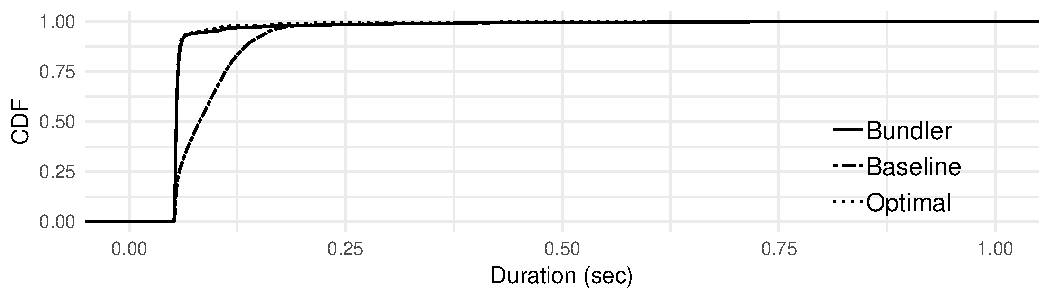
\includegraphics[width=\maxwidth]{figure/eval:best-1} 

\end{knitrout}
    \caption{\name achieves $33$\% lower median slowdown. Note the differing axis scales. For both \name and Optimal, performance benefits come from preventing short flows from queueing behind long ones. \an{Whiskers currently show 1.25 inter-quantile range, figure out how to show 99th \%ile? Also, can barely see Bundler and Optimal...}}
    \label{fig:eval:best}
\end{figure}


We evaluate our implementation of \name (discussed in \S\ref{s:impl}) using network emulation via mahimahi~\cite{mahimahi}.
There are three machines in our setup: one machine is a traffic generator, another is configured as a middlebox, and a third is the receiver.
We run an empirical traffic generator, in which a many-threaded client generates requests from a given request size CDF and sends them to one of $200$ server processes on the traffic generator.
Each server then responds to the client with the requested amount of data.
Note that it is important to use many server processes so that the effect of head-of-line blocking on the client requests is limited.
We then measure the flow completion time of each client request.

We first run \name with no cross traffic.
On a $96$Mbps link, we generate $84$Mbps of offered request load from a simple CDF with a heavy-tailed mix of short and long requests: 90\% of the requests are less than $5$KB, and 100\% of the requests are less than $1$MB. 
In addition, there is a persistently backlogged connection inside the traffic aggregate.
We use a Copa~\cite{copa} congestion controller at the \inbox to manage the bottleneck queue, and the stochastic fair queueing~\cite{sfq} scheduling policy.
The results are in Figure~\ref{fig:eval:best}.
With \name, the median flow completion time (FCT) decreases from $147$ms using FIFO scheduling at the bottleneck link (the baseline configuration) to $58$ms with \name: 61\% lower.

Where do these benefits come from? We devote the remainder of this section to exploring this question.

\paragrapha{Necessity of scheduling} It is important to note that \name is not necessarily a means of achieving low end-to-end delays, as promised by recent efforts in congestion control~\cite{copa, nimbus}. 
To see why this is the case, recall that \name does not modify the end-hosts: they continue to run the default Cubic congestion controller, which will probe for bandwidth until it observes loss.
Indeed, the packets end-host Cubic sends beyond those the link can transmit must queue somewhere in the network or be lost. Without \name, they queue at the bottleneck link.
With \name, they instead queue at the \inbox.

\begin{figure}
    \centering
\begin{knitrout}
\definecolor{shadecolor}{rgb}{0.969, 0.969, 0.969}\color{fgcolor}
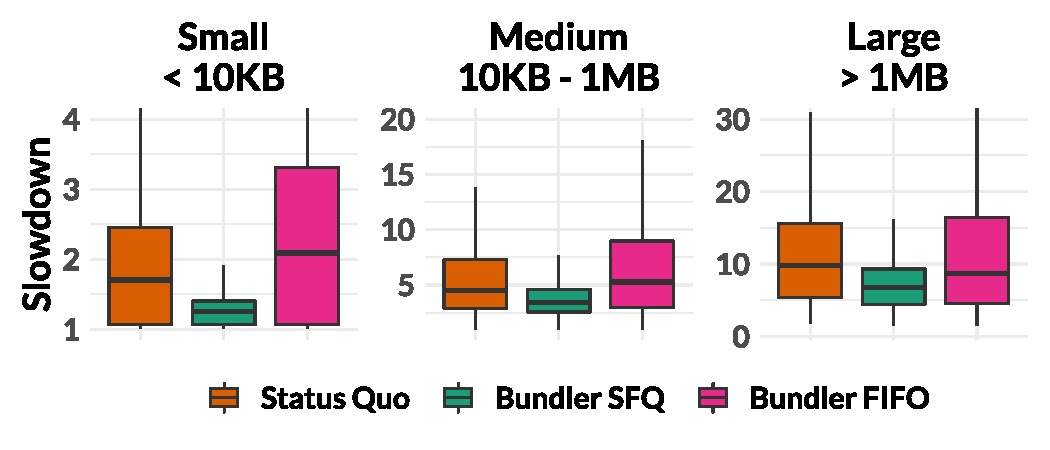
\includegraphics[width=\maxwidth]{figure/eval_fifo-1} 

\end{knitrout}
    \caption{With FIFO scheduling, the benefits of \name are lost: FCTs are 31\% worse in the median. Note the different y-axis scales for each group of request sizes.}
    \label{fig:eval:fifo}
\end{figure}
\newcommand{\overviewBenefitsFifoMedian}{2.13\xspace}
\newcommand{\overviewBenefitsFifoWorse}{31\%\xspace}


We can see this by measuring the relative performance of using FIFO scheduling at the \name compared to the SFQ scheduling in Figure~\ref{fig:eval:best}.
The results are in Figure~\ref{fig:eval:fifo}. 
Unsurprisingly, the FCTs with FIFO scheduling at \name are \emph{worse}: with a median FCT of $173$ms, it is $18$\% worse than the baseline.

\paragrapha{Impact of congestion control} How does our choice of congestion control impact our results? 
It is important to choose a congestion control algorithm carefully based on the known or inferred characteristics of the bottleneck link. 
In Figure~\ref{fig:eval:cc} we show three congestion control protocols: BBR~\cite{bbr}, Nimbus~\cite{nimbus}, and Copa~\cite{copa}.
In this scenario, it is important to control delays. Nimbus and BBR both maintain slightly higher queueing delays at the bottleneck link, and thus they achieve higher median FCTs \an{numbers}.

\begin{figure}
    \centering
\begin{knitrout}
\definecolor{shadecolor}{rgb}{0.969, 0.969, 0.969}\color{fgcolor}
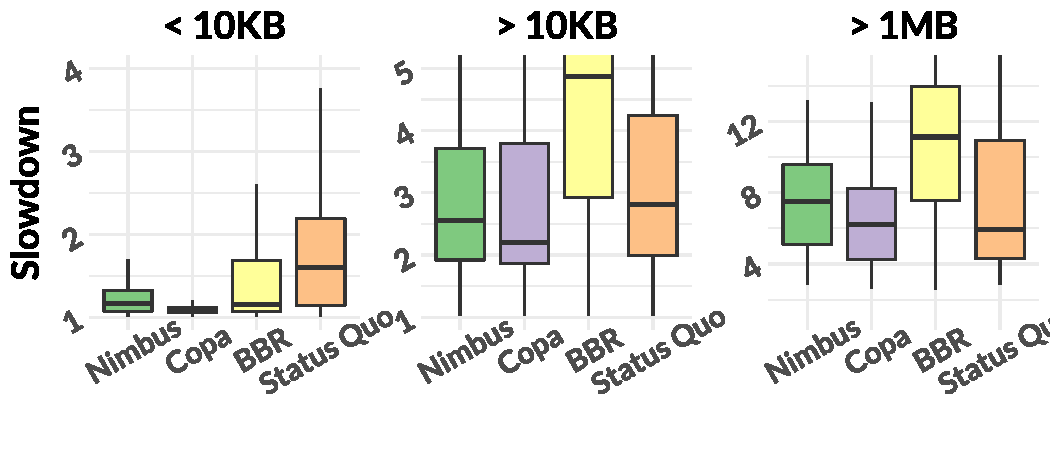
\includegraphics[width=\maxwidth]{figure/eval:cc-1} 

\end{knitrout}
    \caption{Choosing a congestion control algorithm at \name remains important, just as it is at the end-host. Note the different y-axis scales for each group of request sizes.}
    \label{fig:eval:cc}
\end{figure}
\newcommand{\ccCopaMedian}{}
\newcommand{\ccNimbusMedian}{}
\newcommand{\ccBBRMedian}{}
\newcommand{\ccBaselineMedian}{}


\cut{
\begin{outline}[enumerate]
    \1 Bundler can reduce flow completion times
        \2 Base case with no cross traffic: run empirical traffic generator in the bundle varying offered load from 30\% to 90\%
            \3 Rough estimate of current results: 2-3x better for short flows (normalized fct, and only 10-20\% worse for long flows
            \3 Run with and without FQ scheduling, should still see some benefit from scheduling at lower load since there will be spikes of larger flows
            \3 Show how close bundler is to ideal situation (bottleneck router doing FQ scheduling) without actually having to change the middle of the network
        \2 Add inelastic background traffic
        \2 Add elastic background traffic
            \3 Have to enable x-tcp mode (perhaps dynamic number of flows) for bundle
            \3 can measure number of flows by looking at the number of backlogged queues
    \1 Microbenchmarks
        \2 Show that the bundler architecture is capable of emulating rate-based congestion control algorithms: \textbf{PLOT} throughput and delay of Nimbus/BBR/etc with and without bundler show that they look the same and achieve the same average behavior 
            \3 Regardless of underlying number of flows
        \2 Show that the measurements obtained via packet sampling are robust even though epoch size is varying over time due to hashing
        \2 Show why dynamic epoch adjustment is needed 
            \3 If too small relative to rate, there's too much overhead, if too large relative to rate the algorithm can't make progress
            \3 \textbf{PLOT} show BBR with large sampling rate, dies after going into probe RTT because it doesn't get any more measurements 
            \3 Show effect of window of measurements
                \4 important: there are no real ``magic parameters'' here: \name should take measurements in 1-rtt windows, and epochs should be as short as performance considerations allow.
        \2 Standard fairness experiment: 3 background cubic flows not in the bundle, vary the number of flows in the bundle, show that the bundle is able to achieve the "fair" share of the link 
    \1 Bundler allows long running flows to experience better rate stability, the rate of the bundle may fluctuate over time, but long running flows in the bundle see a stable rate while shorter flows 
        \2 Application: could show how this benefits e.g. live video 
    \1 Multiple bundles competing with each other?
    

\end{outline}
}
